\documentclass[10pt,twocolumn,letterpaper]{article}

\usepackage{cvpr}
\usepackage{times}
\usepackage{epsfig}
\usepackage{graphicx}
\usepackage{amssymb}
\usepackage{enumerate}
\usepackage{textcomp}
\usepackage{graphicx}
\usepackage{mathtools}
\graphicspath{ {images/} }

% Include other packages here, before hyperref.
\usepackage{xcolor}
\newcommand\note[1]{\textcolor{red}{#1}}

\usepackage{subcaption}
\usepackage{afterpage}


% If you comment hyperref and then uncomment it, you should delete
% egpaper.aux before re-running latex.  (Or just hit 'q' on the first latex
% run, let it finish, and you should be clear).
\usepackage[breaklinks=true,bookmarks=false]{hyperref}

\cvprfinalcopy % *** Uncomment this line for the final submission

\def\cvprPaperID{****} % *** Enter the CVPR Paper ID here
\def\httilde{\mbox{\tt\raisebox{-.5ex}{\symbol{126}}}}

% Pages are numbered in submission mode, and unnumbered in camera-ready
%\ifcvprfinal\pagestyle{empty}\fi
\setcounter{page}{1}
\begin{document}

%%%%%%%%% TITLE
\title{EECS 442 Computer Vision: Final Project Report}

\author{Nathan Immerman\\
College of Engineering, University of Michigan\\
Ann Arbor, Michigan\\
{\tt\small immerman@umich.edu}
% For a paper whose authors are all at the same institution,
% omit the following lines up until the closing ``}''.
% Additional authors and addresses can be added with ``\and'',
% just like the second author.
% To save space, use either the email address or home page, not both
\and
Alexander Chocron\\
College of Engineering, University of Michigan\\
Ann Arbor, Michigan\\
{\tt\small achocron@umich.edu}
}

\maketitle
%\thispagestyle{empty}

%%%%%%%%% BODY TEXT
\section{Introduction}

With the advent of software tools such as Photoshop and Gimp, it is becoming increasingly simple to doctor and create fake images. One method of doctoring images is to create a composite image out of existing source images. Since composite images are difficult to detect for the common person, we hope to create a tool that enables users to determine composite images.

It is often difficult to make the light direction throughout the entirety of composite images consistent. This fact can be leveraged to detect whether even well-stitched images are fake. By analyzing the light direction of different surfaces within the image, one can detect whether or not the two surfaces came from the same original image. An algorithm for detecting such inconsistencies has been outlined in Johnson and Farid's paper, \emph{Exposing digital forgeries by detecting inconsistencies in lighting}. We shall attempt our own implementation of this algorithm and measure our implementation based on accuracy.

%------------------------------------------------------------------------
\section{Approach}

The equation that we are making use of to estimate the light directions is \[I(x,y) = R\times (\vec{N}(x,y)\cdot \vec{L}) + A\]
where $I(x,y)$ is the intensity at the point $(x,y)$, $R$ is the reflectance term (a constant), and $N(x,y)$ is the unit vector normal to the boundary at the point $(x,y)$. This equation assumes an infinite light source.

A limitation of this equation is that it requires that the reflectance of the surface is known and that it is constant. By assuming that the reflectance equals 1, a vector for the light direction can be obtained with an unknown scale factor. However, this still requires that the object has constant reflectance. As the paper suggests, we are able to relax this constraint by partitioning the boundary into $n$ patches (or partitions), and assume that each of these patches has constant reflectance. We can assume this because small, local patches of an object are likely to be very uniform, and therefore are likely to have a more of a constant reflectance than the overall reflectance of the object. In our implementation, we use $n$ = 8, which the authors of the paper recommend.

\subsection{Finding the Normal Vectors}
To use this algorithm we need to calculate the vectors normal to the object boundaries that are assumed to be given to the algorithm. It is difficult to calculate the normal vector at an arbitrary point on the object because an arbitrary normal vector has three degrees of freedom: one for each component in three dimensions ($x$, $y$, and $z$). To eliminate a degree of freedom and make it possible to calculate the normal vectors, we constrain the algorithm to only consider occluding boundaries because at occluding boundaries, the vector normal to an object surface has a $z$-component of $0$. Also, at the occluding boundary, the $x$ and $y$ components of the normal vectors point in the same direction in both the scene and image coordinates. This makes it possible to estimate the normal vectors without any object-level knowledge or 3D information. 

We estimate a normal vector for each point given in every partition. The object boundary, however, is encoded as a set of points, and it is not possible to compute vectors normal to individual points. To solve this, we fit a quadratic curve $y = p(x)$ for each partition. The curve is fit to three user-selected points $(x_1,y_1), (x_2,y_2), (x_3,x_3)$ that lie near the boundary partition. This process is outlined below in detail:

Given points $(x_1,y_1), (x_2,y_2), (x_3,x_3)$ that correspond to a single partition, we compute the quadratic curve by creating matrices 
\[A = \begin{pmatrix}
		x_1^2 & x_1 & 1\\
		x_2^2 & x_2 & 1\\
		x_3^2 & x_3 & 1
	  \end{pmatrix}\]
\[\vec{y} = \begin{pmatrix}
		y_1\\
		y_2\\
		y_3\end{pmatrix}\]
And then compute
\[\begin{pmatrix} a\\ b\\ c\end{pmatrix} = A^{-1}\vec{y}\]
Where \[p(x) = ax^2 + bx + c.\]

The next step is to compute the vectors normal to the boundary using the quadratic function. For each point $(x,y)$ in the partition, we compute \[m = \frac{-1}{2ax + b}\]
\[N_x(x,y) = \frac{1}{\sqrt{1 + m^2}}\]
\[N_y(x,y) = \frac{m}{\sqrt{1 + m^2}}\]

At each partition, the user must indicate a fourth point that lies on the object to indicate which direction the normal vectors should point. If the normal vector that we calculate points away from this point, we simply scale the normal vector by a factor of -1 to reverse its direction.

\subsection{Estimating Intensities at the Occluding Boundary}
We need to estimate the intensities of the pixels at the occluding boundary because the pixels are not in the image. For a single point along the boundary, this is accomplished by sampling $n$ pixels along the direction opposite of the normal vector and fitting an exponential curve to these values, namely \[I(x) = ax^{b}\] where x is the position along the negative normal direction and $I(0)$ is the intensity at the occluding boundary. We used $n = 15$.

We use basic least-squares estimation on $\log(I(x))$ to determine the parameters $a$ and $b$. The intensity at the occluding boundary is then calculated by evaluating $I(0)$.

\subsection{A Least-Squares Approach For Estimating The Light Directions}
We cannot take a direct approach to solving for the light directions; we have an unknown ambient term and several points in each partition segment. To overcome this, the paper reformulates the problem in such a way that it is possible to apply least squares estimation to solve for the unknowns. After this is complete, we estimate the overall light direction on the object by averaging the light direction of each segment in the partition.

The paper reformulates the problem by first organizing the data:

$(x^{(i)}_j,y^{(i)}_j)$ is the $j$th point of the $i$th partition for a particular boundary. There are $n$ partitions, each of which contains $p$ points.

\[D_k = 
\begin{pmatrix}
N_x(x^{(1)}_1,y^{(1)}_1) & N_y(x^{(1)}_1,y^{(1)}_1) \\
	\vdots & \vdots\\
	N_x(x^{(1)}_p,y^{(1)}_p) & N_y(x^{(1)}_p,y^{(1)}_p) \\
	\end{pmatrix}\]

	
\[M = 
	\begin{pmatrix}
	D_1 & 0 &\cdots & 0 & 1\\
	0 & D_2 &\cdots & 0 & 1\\
 	\vdots & \vdots & \ddots & \vdots& \vdots\\
	0 & 0 & \cdots & D_n & 1\\
	\end{pmatrix}\]
	
	
\[C = 
	\begin{pmatrix}
	-1 & 0 & 1 & 0 & \cdots & 0 & 0 & 0 & 0 & 0\\
	0 & -1 & 0 & 1 & \cdots & 0 & 0 & 0 & 0 & 0\\
	\vdots & & & & \ddots & & & & & \vdots\\
	0 & 0 & 0 & 0 & \cdots & -1 & 0 & 1 & 0 & 0\\
	0 & 0 & 0 & 0 & \cdots & 0 & -1 & 0 & 1 & 0\\
	\end{pmatrix}\]
	
\[\vec{b} =
	\begin{pmatrix}
	I(x^{(1)}_1,y^{(1)}_1)\\
	\vdots\\
	I(x^{(1)}_p,y^{(1)}_p)\\
	\vdots\\
	I(x^{(n)}_1,y^{(n)}_1)\\
	\vdots\\
	I(x^{(n)}_p,y^{(n)}_p)\\
	\end{pmatrix}\]
\[\vec{v} = 
	\begin{pmatrix}
	L^{(1)}_x\\
	L^{(1)}_y\\
	\vdots\\
	L^{(n)}_x\\
	L^{(n)}_y\\
	A\\
	\end{pmatrix}\]
	
$\vec{v}$ is the quantity we are trying to find. To do so, we use this closed form of the least squares optimization:

\[\vec{v} = (M^TM + \lambda C^TC)^+M^T\vec{b}\] where for a matrix $A$, $A^+$ would denote the pseudo-inverse of $A$. This is the closed form equation for finding the least-squares estimate of the light directions. We use $\lambda = 10$, as the paper recommends (for an infinite light source).

%------------------------------------------------------------------------
\section{Implementation}

No third-party software or systems were used. All components of our project, including both the back-end and front-end GUI (graphical user interface), were implemented from scratch (other than built-in functions that MATLAB provides). We chose to implement our tool in MATLAB due to our familiarity with the software and its built-in linear algebra and image manipulation functionality.

Our GUI tries to streamline the user-input phase as much as possible. The steps in using our tool are as follows:

\begin{itemize}
\item The user opens the tool, entering the image path as a command-line argument.

\item The user draws the occluding boundaries at which he or she wishes to determine the light direction. For best results, we recommend using the magnifying glass to zoom in on boundary locations before drawing. The drawings do not need to be perfect, but they should be quite close for best results. As well, the user should be careful to remain on the object and not draw on the background. To initiate the drawing tool, the user must select \emph{Add Boundary}. This process must be repeated for each boundary desired. There is no limit to the number of boundaries that can be drawn. An example boundary can be seen in Figure~\ref{fig:gui1}.

\begin{figure}[]
\begin{center}
	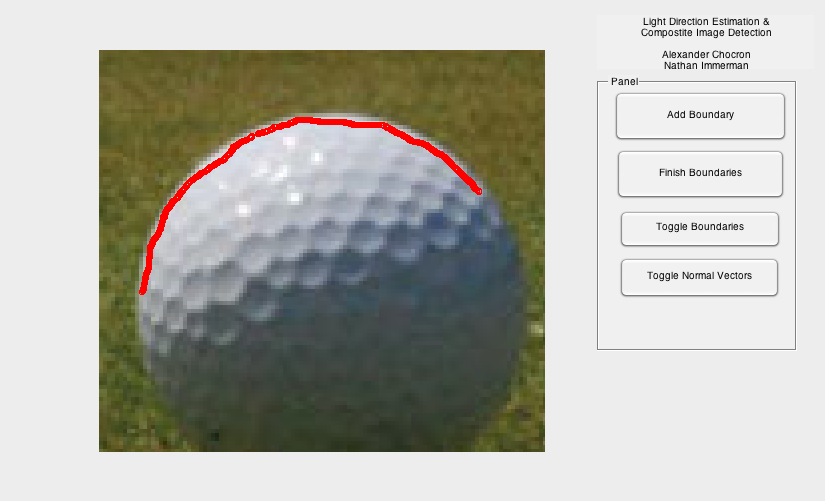
\includegraphics[width=0.9\linewidth]{gui1.png}
\end{center}
	\caption{Adding an occluding boundary.}
\label{fig:gui1}
\end{figure}

\item Once the user is done adding all desired boundaries, he or she must select \emph{Finish Boundaries}. In this phase of the tool, the user will be entering points that are used to estimate a quadric curve to fit to the boundaries that they user added. The GUI zooms in on small patches of a boundary, where the user selects three points that might approximate the small patch. After each set of three points, the user must select a point on the object itself. Once these four points are entered, the GUI zooms in on the next patch. This is repeated for all patches of all boundaries. An example of entering points can be seen in Figure~\ref{fig:gui2}.

\begin{figure}[]
\begin{center}
	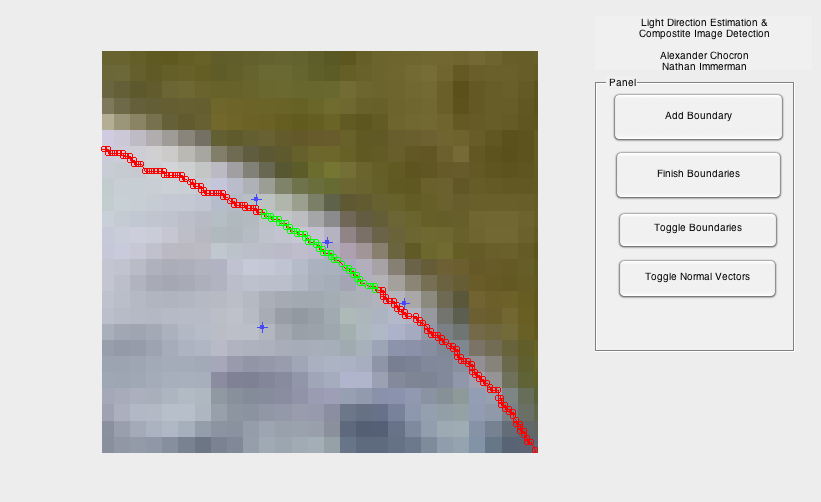
\includegraphics[width=0.9\linewidth]{gui2.png}
\end{center}
	\caption{Adding points (blue) to approximate the boundary.}
\label{fig:gui2}
\end{figure}

\item The GUI then zooms out to reveal the entire boundary and the user selects on the object where the arrow indicating the light direction will be plotted. This process repeats for each boundary that the user added.

\item Finally, the GUI plots the estimated light directions for each boundary at the locations that the user specified

\end{itemize}

The user also has the ability to view the entered boundaries and the estimated normal vectors by toggling the buttons \emph{Toggle Boundaries} and \emph{Toggle Normal Vectors} respectively. Figure~\ref{fig:gui3} shows an estimate light direction show with the yellow arrow, as well as the user entered boundary, shown in red, and the approximated normal vectors, shown in green.

\begin{figure}[]
\begin{center}
	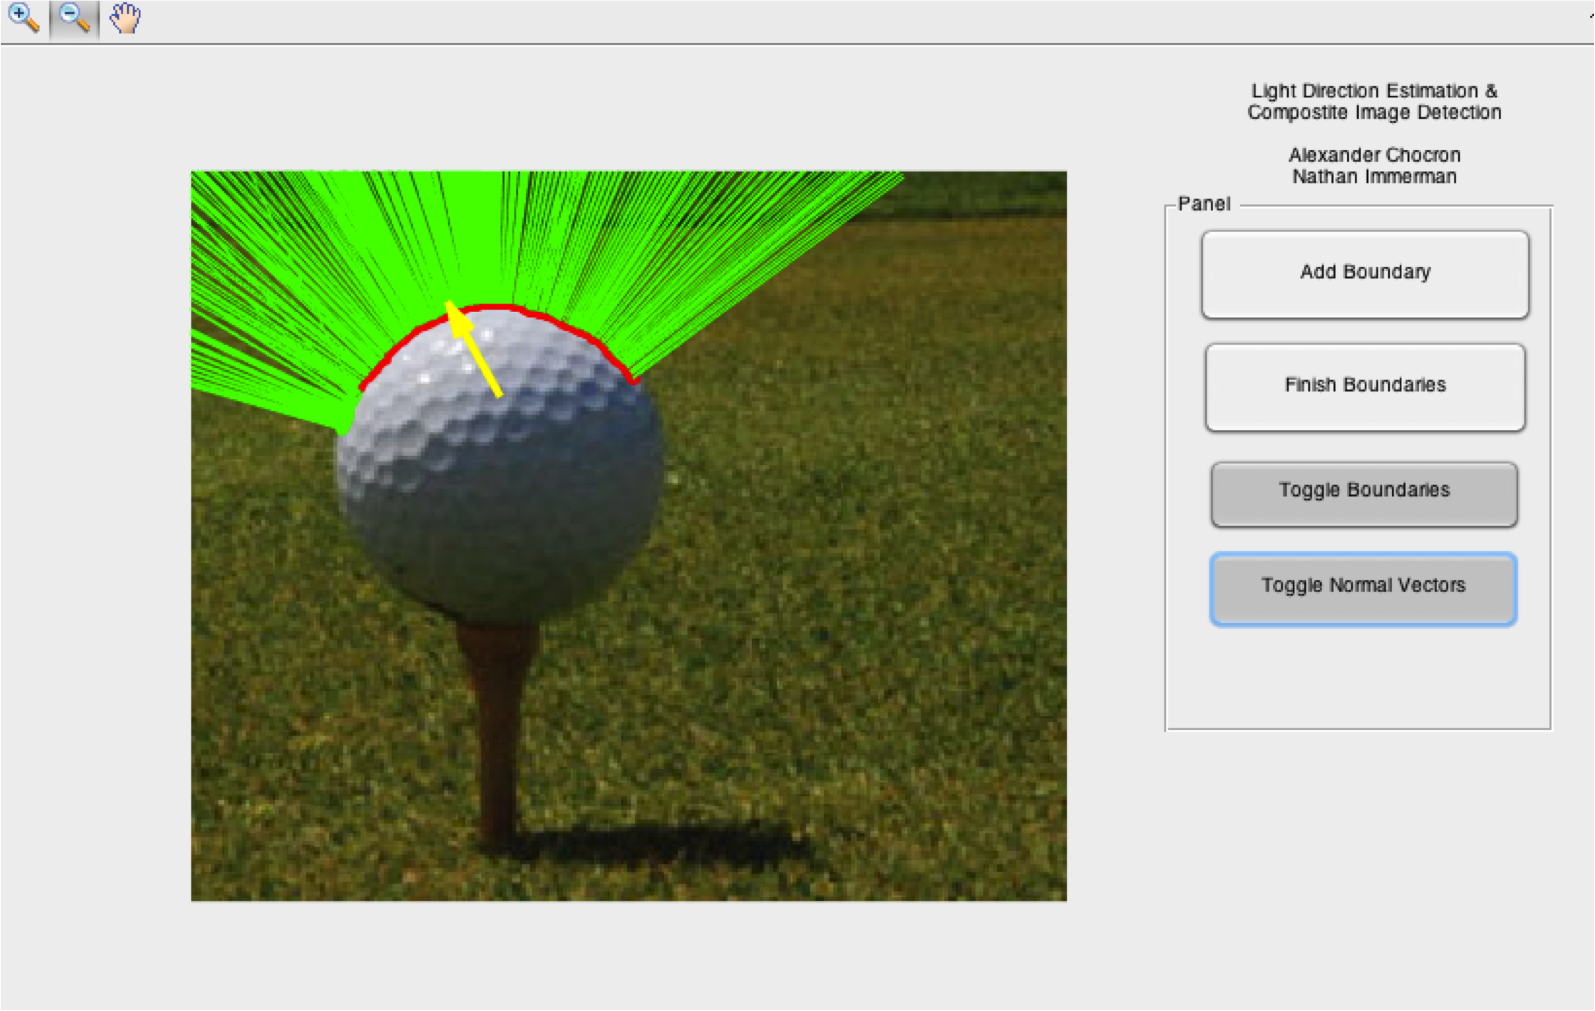
\includegraphics[width=0.9\linewidth]{gui3.png}
\end{center}
	\caption{The estimated light direction (yellow arrow), occluding boundary (red), and approximated normal vectors (green).}
\label{fig:gui3}
\end{figure}

%------------------------------------------------------------------------
\section{Experiments}
We performed a number of experiments to test the performance of our tool. These experiments included both testing the light direction of calculated in images for which a ground truth has been obtained, and testing the tool on known composite images, with an emphasis on the former.

\afterpage{%
	\begin{figure*}[]
	\begin{subfigure}{.5\linewidth}
	  \centering
		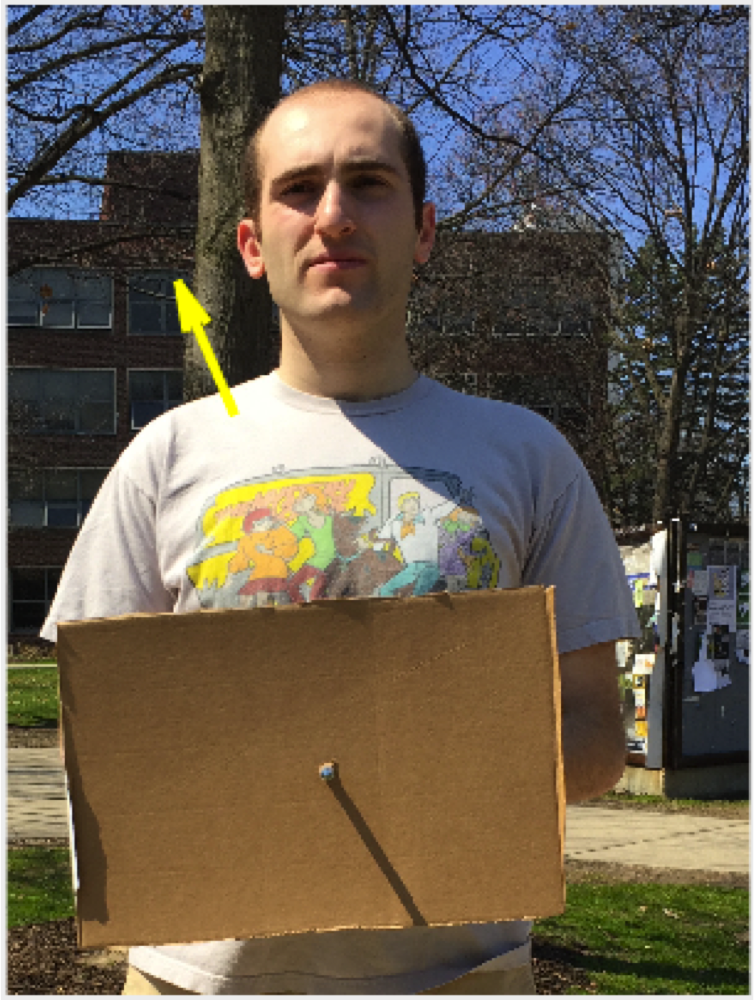
\includegraphics[width=0.5\linewidth]{nathan.png}
	  \caption{}
	  \label{fig:sfig1}
	\end{subfigure}
	\begin{subfigure}{.5\linewidth}
	  \centering
		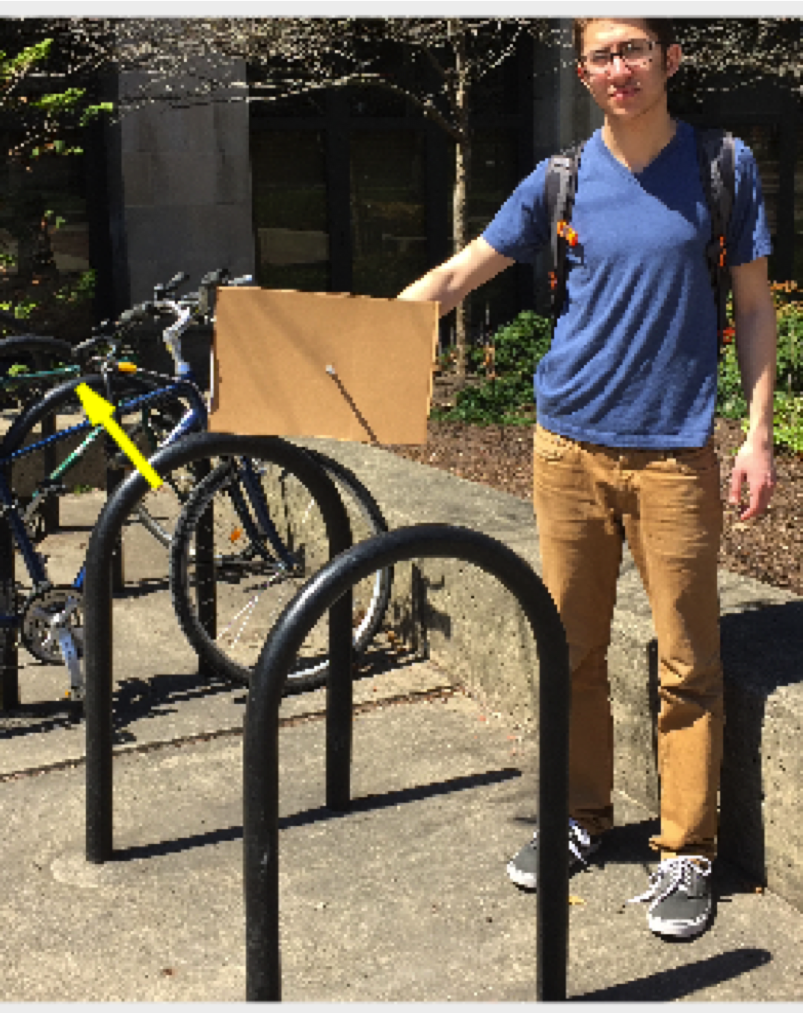
\includegraphics[width=0.5\linewidth]{zander.png}
	  \caption{}
	  \label{fig:sfig2}
	\end{subfigure}
	\begin{subfigure}{.5\linewidth}
	  \centering
		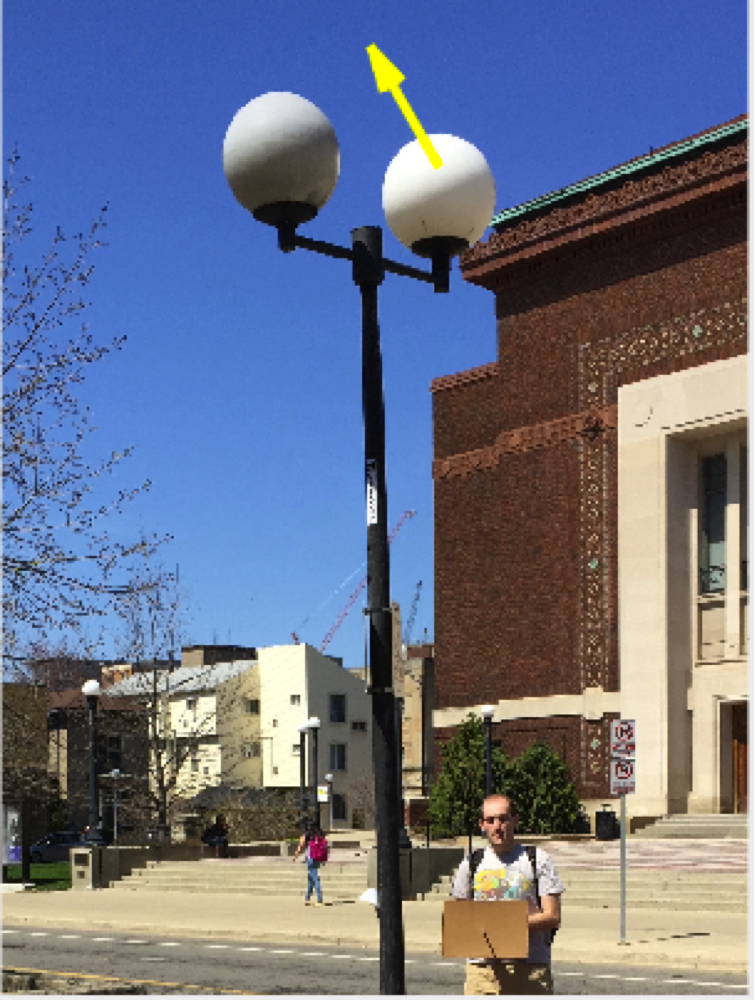
\includegraphics[width=0.5\linewidth]{lamppost.png}
	  \caption{}
	  \label{fig:sfig3}
	\end{subfigure}
	\begin{subfigure}{.5\linewidth}
	  \centering
		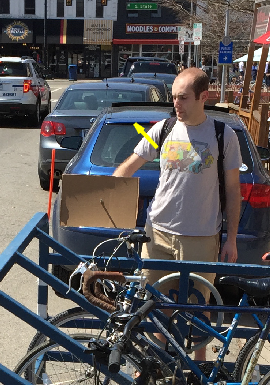
\includegraphics[width=0.5\linewidth]{bike_rack_1.png}
	  \caption{}
	  \label{fig:sfig4}
	\end{subfigure}
	\begin{subfigure}{.5\linewidth}
	  \centering
		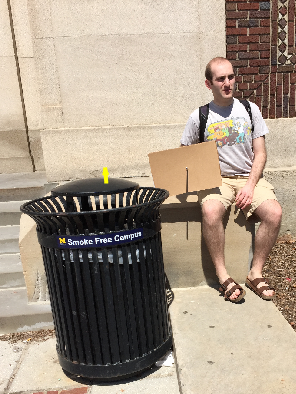
\includegraphics[width=0.5\linewidth]{garbage_can.png}
	  \caption{}
	  \label{fig:sfig5}
	\end{subfigure}
	\begin{subfigure}{.5\linewidth}
	  \centering
		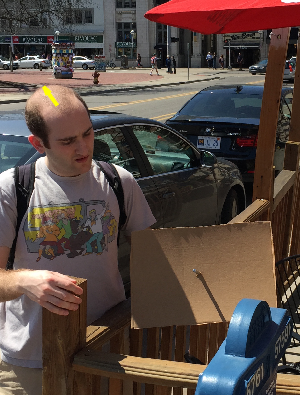
\includegraphics[width=0.5\linewidth]{nathan_2.png}
	  \caption{}
	  \label{fig:sfig6}
	\end{subfigure}
	\caption{Images taken that with known light directions.}
	\label{fig:images}
	\end{figure*}
	\clearpage
}
% \newpage
\subsection{Images with Known Light Directions}
In Figure~\ref{fig:images} are examples of images that we tested our tool on. The ground truth for the light direction was estimated by holding a board with a protruding rod parallel to the image plane and measuring the direction of the shadow cast by the sun. This was then compared to the output of our tool. A brief summary of our results:
\\\\
\begin{tabular}{c | c | c | c }

Image & Est. Direction & Ground Truth & Difference\\
\hline
(a) & 121\textdegree & 113\textdegree & 8\textdegree\\
(b) & 122\textdegree & 128\textdegree & 6\textdegree\\
(c) & 115\textdegree & 120\textdegree & 5\textdegree\\
(d) & 133\textdegree & 120\textdegree & 13\textdegree\\
(e) & 95\textdegree & 89\textdegree & 6\textdegree\\
(f) & 126\textdegree & 119\textdegree & 7\textdegree\\
\end{tabular}
\\\\
Angles are measured South of West.\\\\
The average error for these images is 7.5\textdegree. We find that different kinds of surfaces yield different results. Typically, shirt sleeves, spherical objects, and fairly solid-colored objects give the best results. The algorithm makes a Lambertian assumption, so the less spectral reflection the better the tool performs (but sometimes surprisingly good results are obtained with shiny objects).

\subsection{Composite Photo Analysis}
Figure~\ref{img:golfFake} is an example of a composite image that our tool performs quite well with. An image of a golf ball has been placed on the bulb on the left, and the tool calculates a light direction discrepancy of 69\textdegree, strongly (and correctly) indicating a forgery.

\begin{figure}[htpb]
\begin{center}
	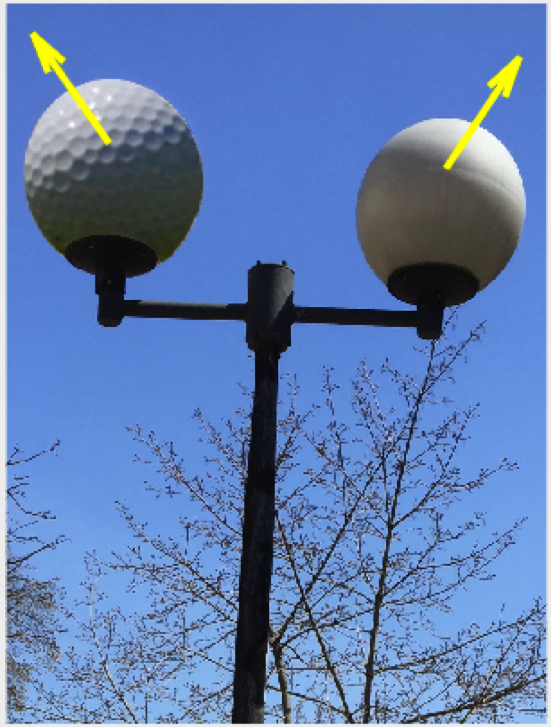
\includegraphics[width=0.9\linewidth]{golfball_fake_labeled.png}
\end{center}
	\caption{An example of a composite (fake) image where there is clearly a light discrepancy. Our tool exposed a light direction difference of 69\textdegree.}
\label{img:golfFake}
\end{figure}

\subsection{Error Analysis}
Our tool requires a significant amount of user input which we believe is our major source of error. If the user does not choose points or draw the boundary carefully, the results may be significantly skewed. We sometimes had to try multiple times to achieve positive results on a single image. Another source of error might be jpeg compression artifacts. We believe best results would be obtained with an uncompressed image format, because compression artifacts might significantly obscure the pixels near boundaries. Further, we make a Lambertian assumption, however, this is not always accurate for many objects.

%------------------------------------------------------------------------
\section{Conclusion and Future Work}
By implementing the algorithm in Johnson and Farid's paper, \emph{Exposing digital forgeries by detecting inconsistencies in lighting}, we were able to produce robust estimates of light directions and detect composite images. On images that we took outside on a sunny day we were able to achieve average error of 7.5\textdegree. Based on this result we would classify an image as a forgery if the image has two light directions with a discrepancy of over 25\textdegree. 
 
Light directions are often a reliable way to detect forgeries, however, the method is somewhat limited. Many images are not well-suited for this kind of detection, whether they lack suitable surfaces or the user simply does not know what he or she is looking for. In order to make use of the tool, the user must select boundaries on portions of the image that are suspected of being stitched together. We hope to incorporate other forgery detection algorithms that would account for more conditions to create an even more robust tool.

In addition, we hope to remove many of the user input elements of the algorithm by finding a way to algorithmically obtaining the occluding boundaries. We also hope to implement an extended version that works in local lighting.
%--------------------------------	----------------------------------------
\section{References}

[1] M. K. Johnson and H. Farid. Exposing digital forgeries by detecting inconsistencies in lighting. \emph{In Proceedings of the 7th workshop on Multimedia and security}, pages 1-10, 2005.

\end{document}
